%%%%%%%%%%%%%%%%%%%%%%%%%%%%%%%%%%%%%%%%%%%%%%%%%%%%%%%%%%%%%%%%%%%%%%%%%%%%%%%%
% Front matter
%%%%%%%%%%%%%%%%%%%%%%%%%%%%%%%%%%%%%%%%%%%%%%%%%%%%%%%%%%%%%%%%%%%%%%%%%%%%%%%%

\title{partial: An R Package for Creating Partial Dependence Plots}
\author{by Brandon M. Greenwell}

\maketitle

\abstract{
Complex nonparametric models (e.g., neural networks, random forests, and support vector machines) are often used in predictive analytics, especially when dealing with large observational databases that don't adhere to the strict assumptions imposed by traditional statistical techniques (e.g. multiple linear regression). Unfortunately, it can be challenging for the uninitiated to understand the results of such models and explain them to management. Partial dependence plots offer a simple solution. Partial dependence plots are low-dimensional graphical renderings of the prediction function $\widehat{f}\left(\boldsymbol{x}\right)$ so that the relationship between the outcome and predictors of interest can be easily understood. These plots are especially useful in explaining the output from complex black box models like support vector machines or neural networks or constructing simpler parsimonious models on newly obtained data.
}


%%%%%%%%%%%%%%%%%%%%%%%%%%%%%%%%%%%%%%%%%%%%%%%%%%%%%%%%%%%%%%%%%%%%%%%%%%%%%%%%
% Introduction
%%%%%%%%%%%%%%%%%%%%%%%%%%%%%%%%%%%%%%%%%%%%%%%%%%%%%%%%%%%%%%%%%%%%%%%%%%%%%%%%
\section{Introduction}

Predictor importance is an important task in any supervised learning problem. However, ranking variables is only part of the story and once a subset of "important" features is identified it is often necessary to assess the relationship between them (or subset thereof) and the response. This can be done in many ways, but in machine learning it is often accomplished by constructing \dfn{partial dependence plots} (PDPs); see \citet{friedman-2000-greedy} for details. PDPs help visualize the relationship between a subset (typically 1-3) of the predictors and the response while accounting for the average effect of the other independent variables in the model. They are particularly effective with black box models like random forest and support vector machines.
%PDPs offer a low-dimensional graphical rendering of the prediction function $\widehat{f}\left(\boldsymbol{x}\right)$ for any type of fitted models and are especially useful in visualizing the relationships discovered by complex machine learning algorithms such as a \dfn{random forest}.

Let $\boldsymbol{x} = \left\{x_1, x_2, \dots, x_n\right\}$ represent the predictors in a model whose prediction function is $\widehat{f}\left(\boldsymbol{x}\right)$. If we partition $\boldsymbol{x}$ into an interest set, $\boldsymbol{z}_s$, and its compliment, $\boldsymbol{z}_{c} = \boldsymbol{x} \setminus \boldsymbol{z}_s$, then the partial dependence of the response on $\boldsymbol{z}_s$ is defined as
\begin{equation}
\label{eqn:pdf}
\bar{f}_s\left(\boldsymbol{z}_s\right) = \frac{1}{n}\sum_{i = 1}^n\widehat{f}\left(\boldsymbol{z}_s,\boldsymbol{z}_{i, c}\right),
\end{equation}
where $\boldsymbol{z}_{i, c}$ $\left(i = 1, 2, \dots, n\right)$ are the values of $\boldsymbol{z}_c$ that occur in the training sample; that is, weaverage out the effects of all the other predictors in the model. Let $x_1$ be the predictor variable of interest with unique values $\left\{x_{11}, x_{12}, \dots, x_{1k}\right\}$. The partial dependence of the response on $x_1$ can be constructed as follows:
\begin{enumerate}
  \item For $i \in \left\{1, 2, \dots, k\right\}$:
  \begin{enumerate}
    \item Create a copy of the training data and replace the original values of $x_1$ with the constant $x_{1i}$.
    \item Compute the vector of predicted values from the modified copy of the training data.
    \item Compute the average prediction to obtain $\bar{f}_1\left(x_{1i}\right)$.
  \end{enumerate}
  \item Plot the pairs $\left[x_{1i}, \bar{f}_1\left(x_{1i}\right)\right]$ for $i = 1, 2, \dotsc, k$.
\end{enumerate}
This can be quite computationally intensive since the algorithm involves $k$ passes over the training records. Fortunately, this can be parallelized quite easily. This algorithm can also be easily extended to larger subsets of 2 or more features as well.

Limited implementations of Friedman's PDPs are available in packages \CRANpkg{randomForest} \citep{randomForest-pkg} and \CRANpkg{gbm}, among others; these are limited in the sense that they only apply to the models fit using these packages. For example, the \code{partialPlot} function in \pkg{randomForest} only applies to objects of class \code{"randomForest"}. While the \pkg{randomForest} implementation will only allow for a single predictor, the \pkg{gbm} implementation can deal with any subset of the predictor space; however, these implementations only apply to models fit using the respective package. Partial dependence functions are not restricted to tree-based models; they can be applied to any supervised learning algorithm (e.g., neural networks). However, to our knowledge, there is no general package for constructing PDPs  in R (e.g., PDPs for a \dfn{conditional random forest} as implemented by the \code{cforest} function in the \CRANpkg{party} and \CRANpkg{partykit} packages; see \citet{party-pkg} and \citet{partykit-pkg}, respectively). The \CRANpkg{partial} \citep{partial-pkg} package tries to close this gap by offering a general framework for PDPs that can be applied to several types of fitted models.

The \CRANpkg{plotmo} package \citep{plotmo-pkg} is one alternative to \pkg{partial}. According to the author, \pkg{plotmo} constructs "a poor man's partial dependence plot." In particular, it plots a model's response when varying one or two predictors while holding the other predictors in the model constant (continuous features are fixed at their median value, while factors are held at their first level). These plots allow for up to two variables at a time and are less accurate than PDPs, but are faster to construct. For additive models (i.e., no interactions), these plots are identical in shape to partial dependence plots.

PDPs can be misleading in the presence of substantial interactions \citep{goldstein-peeking-2015}. To overcome this issue \citeauthor*{goldstein-peeking-2015} developed the concept of \dfn{individual conditional expectation} (ICE) plots -- available in the \CRANpkg{ICEbox} package. \pkg{ICEbox} only allows for one variable at a time (i.e., no multivariate displays), though color can be used effectively to display information about an additional predictor. The ability to construct derivative plots is also available.

Many other techniques exist for visualizing relationships between the predictors and the response based on a fitted model. For example, the \CRANpkg{car} package \citep{fox-car-2011} contains many functions for constructing partial-residual and marginal-model plots. The \CRANpkg{effects} package \citep{fox-effects-2003} is also of interest. However, these methods are orientated towards simpler parametric models (e.g., linear and generalized linear models), whereas \pkg{plotmo}, \pkg{ICEbox}, and \pkg{partial} are mainly for nonparametric and black box models (though they can be used for simple parametric models as well).


%%%%%%%%%%%%%%%%%%%%%%%%%%%%%%%%%%%%%%%%%%%%%%%%%%%%%%%%%%%%%%%%%%%%%%%%%%%%%%%%
% PDPs in R
%%%%%%%%%%%%%%%%%%%%%%%%%%%%%%%%%%%%%%%%%%%%%%%%%%%%%%%%%%%%%%%%%%%%%%%%%%%%%%%%
\section{Constructing PDPs in R}

As described in the introduction, the \pkg{partial} package is useful for constructing PDPs for many types of fitted models in R. These are especially useful for visualizing the relationships discovered by complex machine learning algorithms such as a random forest. The latest stable release is available from \href{https://cran.r-project.org/package=partial}{CRAN}:
\begin{example}
install.packages("partial")
\end{example}
The development version is located on GitHub: \url{https://github.com/bgreenwell/partial}. Bug reports and usggestions are appreciated and should be sumbitted to \url{https://github.com/bgreenwell/partial/issues}.

Currently, only two functions are exported by \pkg{partial}:
\begin{itemize}
  \item \code{partial}
  \item \code{plotPartial}
\end{itemize}
The \code{partial} function evaluates the partial dependence \eqref{eqn:pdf} from a fitted model over a grid of predictor values. If \code{plot = FALSE} (the default), \code{partial} returns a data frame with an additional class: \code{"partial"}. The columns are labeled in the same order as the features supplied to \code{pred.var}, and the last column is always labeled \code{y} and contains the partial dependence function values $\bar{f}_s\left(\boldsymbol{z}_s\right)$. If \code{plot = TRUE}, then \code{partial} returns a \CRANpkg{lattice} plot \citep{lattice-pkg}. For more advanced plotting, the \code{plotPartial} function will take a \code{"partial"} object and display a more customizable lattice plot. 

Currently supported models are described in Table~\ref{tab:models}. While more models will be added, the \code{partial.default} method should be able to handle many others not listed in Table~\ref{tab:models}; for example, neural networks from the \CRANpkg{nnet} package \citep{venables-modern-2002} or projection pursuit regression \citep{friedman-ppr-1981} using the \code{ppr} function in the \pkg{stats} package.
\begin{table}[htbp]
  \begin{tabular}{p{4cm}ll}
    \toprule
      Type of model & R package & Object class \\
      \midrule
      Decision trees            & \CRANpkg{rpart} \citep{rpart-pkg} & \code{"rpart"} \\
                                & \pkg{party}    & \code{"BinaryTree"} \\
                                & \pkg{partykit} & \code{"constparty"}/\code{"party"} \\
      Bagged decision trees     & \CRANpkg{ipred} \citep{ipred-pkg} & \code{"classbagg"}, \code{"regbagg"} \\
                                & \CRANpkg{adabag} \citep{adabag-pkg} & \code{"bagging"} \\
      Boosted decision trees    & \pkg{gbm}      & \code{"gbm"} \\
                                & \CRANpkg{adabag} \citep{adabag-pkg} & \code{"boosting"} \\
      Random forest & \pkg{randomForest} & \code{"randomForest"} \\
      Conditional random forest & \pkg{party}    & \code{"RandomForest"} \\
                                & \pkg{partykit} & \code{"cforest"} \\
      Linear model              & \pkg{stats}    & \code{"lm"} \\
      Generalized linear model  & \pkg{stats}    & \code{"glm"}, \code{"lm"} \\
      Multivariate adaptive regression splines (MARS) & \CRANpkg{earth} \citep{earth-pkg} & \code{"earth"} \\
      Support vector machines   & \CRANpkg{e1071} \citep{e1071-pkg} & \code{"svm"} \\
                                & \CRANpkg{kernlab} \citep{kernlab-pkg} & \code{"ksvm"} \\
      \bottomrule
  \end{tabular}
  \caption{Models specifically supported by the \pkg{package}.}
  \label{tab:models}
\end{table}

For illustration, we will use the (corrected) Boston housing data which are available from the \CRANpkg{mlbench} package \citep{mlbench-pkg}. These data contain the median value of owner-occupied homes in 506 U.S. census tracts in the Boston area, along with 13 independent variables such as the per capita crime rate by town. We begin by loading the data and omitting unimportant columns.
\begin{example}
data(BostonHousing2, package = "mlbench")  # mlbench must be installed!
boston <- BostonHousing2[, -c(1, 2, 5)]
\end{example}
Next, we fit a random forest to the entire data set with default tuning parameters and 500 trees:
\begin{example}
library(randomForest)
set.seed(101)  # for reproducibility
boston.rf <- randomForest(cmedv ~ ., data = boston, importance = TRUE)
varImpPlot(boston.rf)  # variable importance plot
\end{example}
The model fit is reasonable, with an \dfn{out-of-bag} (pseudo) $R^2$ of 0.89. The variable importance scores are displayed in Figure~\ref{fig:plotmo_vs_partial}. Both plots indicate that the percentage of lower status of the population (\code{lstat}) and the average number of rooms per dwelling (\code{rm}) are highly associated with the median value of owner-occupied homes (\code{cmedv}). The question then arises, "What is the nature of these associations?" To help answer this, we can look at the partial dependence of \code{cmedv} on \code{lstat} and \code{rm}, both individually and together.

\begin{figure}[htbp]
  \centering
  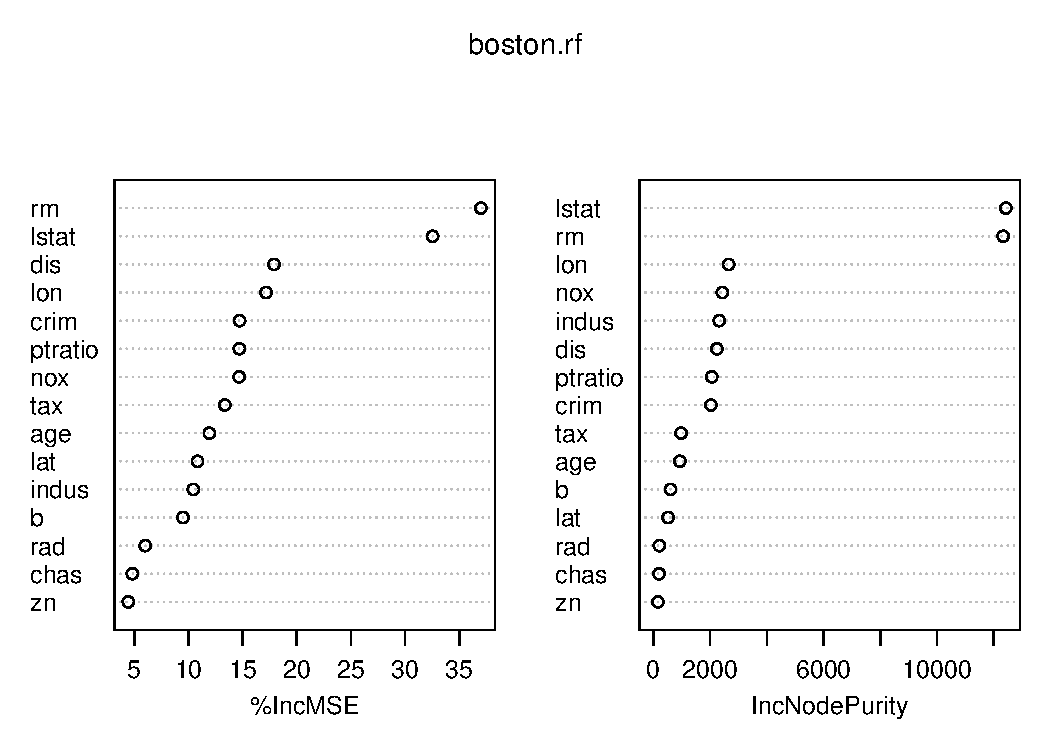
\includegraphics[width=1.0\linewidth]{boston_rf_vimp}
  \caption{Dotchart of variable importance scores for the Boston housing data based on a random forest with 500 trees.}
  \label{fig:plotmo_vs_partial}
\end{figure}


%%%%%%%%%%%%%%%%%%%%%%%%%%%%%%%%%%%%%%%%%%%%%%%%%%%%%%%%%%%%%%%%%%%%%%%%%%%%%%%%
% Univariate PDPs
%%%%%%%%%%%%%%%%%%%%%%%%%%%%%%%%%%%%%%%%%%%%%%%%%%%%%%%%%%%%%%%%%%%%%%%%%%%%%%%%
\subsection{Single predictor PDPs}

As previously mentioned, the \code{randomForest} package has its own \code{partialPlot} function for visualizing the partial dependence of the response on a single predictor. For example, the following snippet of code plots the partial dependence of \code{cmedv} on \code{lstat}:
\begin{example}
partialPlot(boston.rf, pred.data = boston, x.var = "lstat")
\end{example}
The same plot can be achieved using the \code{partial} function and setting \code{plot = TRUE} (see the left side of Figure~\ref{fig:pd_lstat}):
\begin{example}
library(partial)
partial(boston.rf, pred.var = "lstat", plot = TRUE)
\end{example}
The only difference is that \pkg{partial} uses the \pkg{lattice} graphics package to produce all of its displays.

For a more customizable plot, call \code{partial} with \code{plot = FALSE} and use the \code{plotPartial} function. \strong{Note:} the \dfn{pipe} operator \code{\%>\%} provided by the \CRANpkg{magrittr} package \citep{magrittr-pkg} is exported for writing more convenient code, as illustrated in snippet of code below which increases the line width, adds a LOESS smoother, and customizes the $y$-axis label.
\begin{example}
boston.rf %>%
  partial(pred.var = "lstat") %>%
  plotPartial(smooth = TRUE, lwd = 2, ylab = expression(f(lstat)))
\end{example}
The result is displayed in the right side of Figure~\ref{fig:pd_lstat} below.

\begin{figure}[htbp]
  \centering
  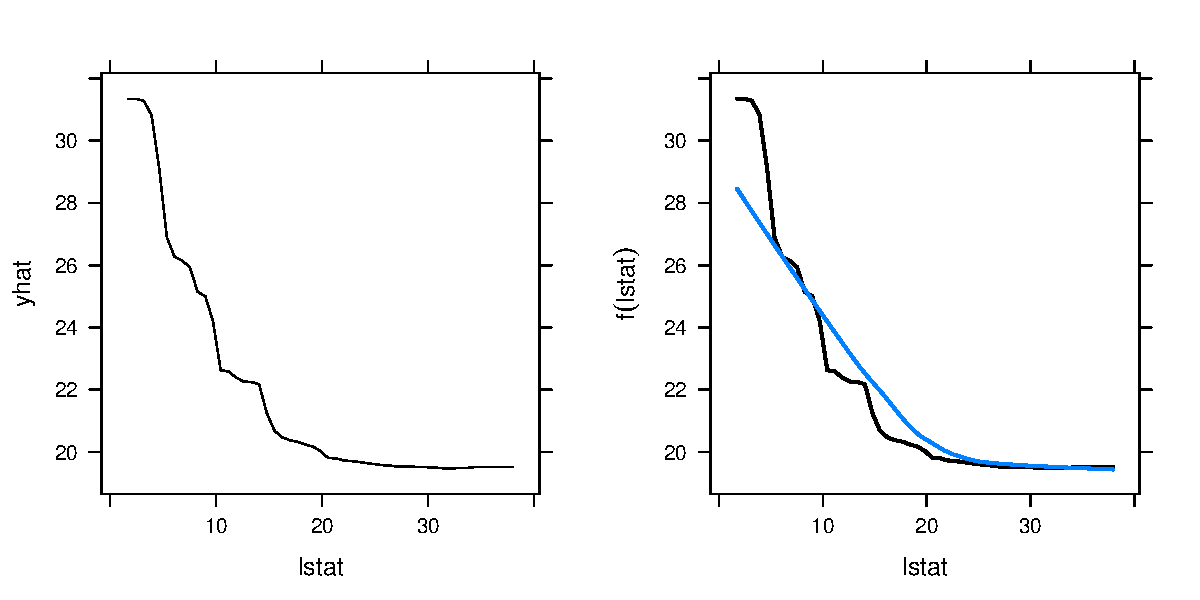
\includegraphics[width=1.0\linewidth]{pd_lstat}
  \caption{Partial dependence of \code{cmedv} on \code{lstat} based on a random forest. \textit{Left}: Default plot. \textit{Right}: Customized plot obtained using the \code{plotPartial} function.}
  \label{fig:pd_lstat}
\end{figure}


%%%%%%%%%%%%%%%%%%%%%%%%%%%%%%%%%%%%%%%%%%%%%%%%%%%%%%%%%%%%%%%%%%%%%%%%%%%%%%%%
% Higher order PDPs
%%%%%%%%%%%%%%%%%%%%%%%%%%%%%%%%%%%%%%%%%%%%%%%%%%%%%%%%%%%%%%%%%%%%%%%%%%%%%%%%
\subsection{Multi-predictor PDPs}

The benefit of using \code{partial} is threefold: (1) it is a generic function that can be used for various types of model fits (not just random forests), (2) it will allow for any number of predictors to be used, and (3) it can utilize any of the parallel backends supported by the \CRANpkg{foreach} package \citep{foreach-pkg}; we discuss parallel execution in a later section. For example, the following code chunk could be used to assess the joint effect of \code{lstat} and \code{rm} on \code{cmedv} based on a conditional random forest using various options in \code{plotPartial}. The results are displayed in Figure~\ref{fig:pd_lstat_rm}.
\begin{example}
library(party)
boston.crf <- cforest(cmedv ~ ., data = boston)
pd.lstat.rm <- partial(boston.crf, pred.var = c("lstat", "rm"))
plotPartial(pd.lstat.rm)
plotPartial(pd.lstat.rm, col.regions = colorRampPalette(c("white", "blue")))
plotPartial(pd.lstat.rm, contour = FALSE, zlab = "cmedv", drape = TRUE,
            colorkey = TRUE, screen = list(z = -20, x = -60))
\end{example}
Note that the default color map for contour plots is the Matplotlib "viridis" color map provided through the \CRANpkg{viridis} package \citep{viridis-pkg}.

\begin{widefigure}[htbp]
  \centering
  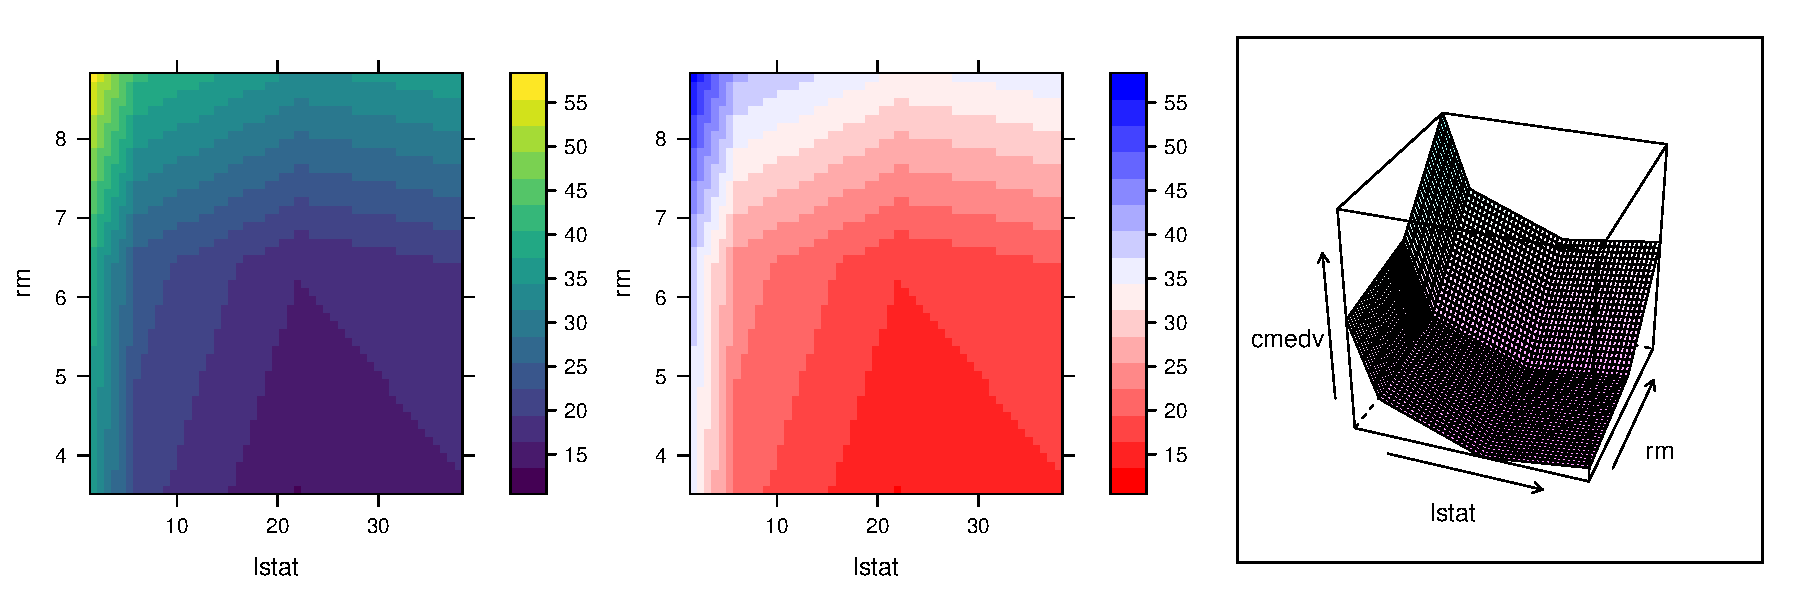
\includegraphics[width=1.0\linewidth]{pd_lstat_rm}
  \caption{Partial dependence of \code{cmedv} on \code{lstat} and \code{rm} based on a conditional random forest. \textit{Left}: Default plot. \textit{Middle}: Using a different color palette. \textit{Right}: Using a 3-D surface.}
  \label{fig:pd_lstat_rm}
\end{widefigure}

% \sub\subsection{Multiple linear regression}
% Here we use the multivariate adaptive regression splines (See ????) algorithm to perform multiple linear regression with automatc variable selection and interaction detection.
% \begin{example}
% library(earth)
% boston.mars <- earth(cmedv ~ ., data = boston, degree = 3, linpreds = TRUE,
%                      pmethod = "exhaustive")
% partial(boston.mars, pred.var = c("nox", "rm"), grid.resolution = 10)
% \end{example}


%%%%%%%%%%%%%%%%%%%%%%%%%%%%%%%%%%%%%%%%%%%%%%%%%%%%%%%%%%%%%%%%%%%%%%%%%%%%%%%%
% Avoiding extrapolation
%%%%%%%%%%%%%%%%%%%%%%%%%%%%%%%%%%%%%%%%%%%%%%%%%%%%%%%%%%%%%%%%%%%%%%%%%%%%%%%%
\subsection{Avoiding extrapolation}

There are a few ways to mitigate the risk of extrapolation in PDPs: rug displays and convex hulls. Rug displays are one-dimensional plots added to the axes. \code{plotPartial} has a \code{rug} option that will display the deciles of the distribution (as well as the minimum and maximum values) for the predictors on the horizontal and/or vertical axes. The following snippet of code produces the left display in Figure~\ref{fig:partial_extrap}. %Notice that in both examples we had to provide the original training data to \code{plotPartial} via the \code{train} option.
\begin{example}
partial(boston.rf, pred.var = "lstat", rug = TRUE, plot = TRUE)
\end{example}

In higher dimensions, plotting the convex hull is more informative; it outlines the region of the predictor space that the model was trained on. When \code{chull = TRUE}, the convex hull of the first two dimensions of $\boldsymbol{z}_s$ (i.e., the first two variables supplied to \code{pred.var}) is added to the plot; alternatively, you can set \code{chull = TRUE} in the call to \code{partial}, in which case only the region within the convex hull of the first two variables is plotted. Over interpreting the partial dependence plot outside of this region can be dangerous. The right right display in Figure~\ref{fig:partial_extrap} was produced using:
\begin{example}
partial(boston.rf, pred.var = c("lstat", "rm"), chull = TRUE, plot = TRUE)
\end{example}

\begin{figure}[htbp]
  \centering
  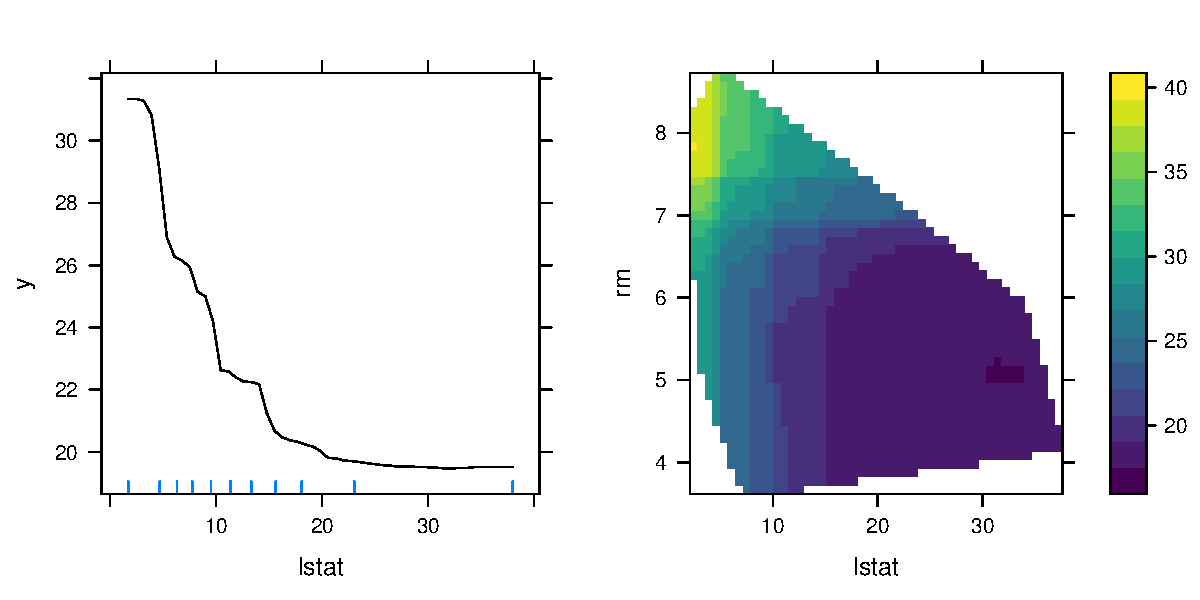
\includegraphics[width=1.0\linewidth]{partial_extrap}
  \caption{Examples of partial dependence plots with the addition of a rug display (left) and a convex hull (right).}
  \label{fig:partial_extrap}
\end{figure}

\subsection{Addressing computational concerns}

Constructing PDPs can be quite computationally expensive. Additional options are available to ease the computational intensity for large problems. For example, there is no need to compute partial dependence of median home value using each unique value of \code{rm} in the training data (which would require 446 passes over the data!). We could get very reasonable results using a reduced number of points. Current options are to use a grid of equally spaced values in the range of the variable of interest; the number of points ban be controlled using the \code{n.pts}. Alternatively, a specific set of values (e.g., quantiles of interest) can be supplied through the \code{pred.grid} argument. To illustrate, the following snippet of code computes the partial dependence of median home value on \code{rm} using each option; the results are displayed in Figure~\ref{fig:partial_manual}.
\begin{example}
partial(boston.rf, plot = TRUE)
partial(boston.rf, "rm", grid.resolution = 30, plot = TRUE)
partial(boston.rf, "rm", pred.grid = data.frame(rm = 3:9), plot = TRUE)
\end{example}

\begin{widefigure}[htbp]
  \centering
  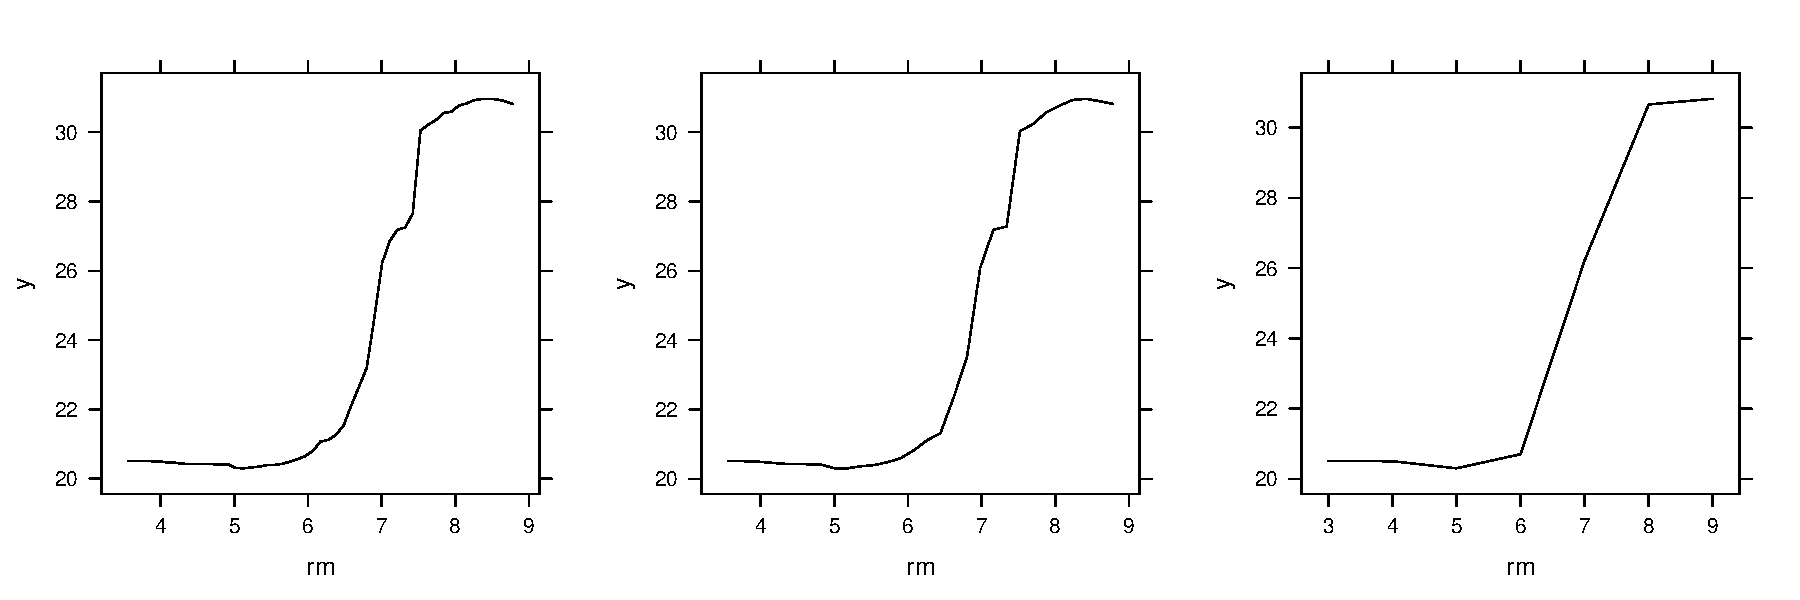
\includegraphics[width=0.8\linewidth]{partial_manual}
  \caption{Partial dependence of \code{cmedv} on \code{rm}. \textit{Left}: Default plot. \textit{Middle}: Using a reduced grid size. \textit{Right}: Using a user-specified grid.}
  \label{fig:partial_manual}
\end{widefigure}

The \code{partial} function relies on the \CRANpkg{plyr} package \citep{plyr-pkg}, rather than for loops. This makes it possible to request progress bars (e.g., \code{.progress = "text"}) or run \code{partial} in parallel. In fact, \code{partial} can use any of the parallel backends supported by the \pkg{foreach} package. To use this functionality, we must load and register a supported parallel backend (e.g., \CRANpkg{doMC} \citep{doMC-pkg} or \CRANpkg{doParallel} \citep{doParallel-pkg}). The following snippet of code obtains the partial dependence of median home value on \code{rm}, \code{lstat}, and \code{ptratio} in parallel. The result is displayed in Figure~\ref{fig:partial_par}.

Setting up a parallel backend is rather straightforward. To illustrate, the following snippet of sets up the \code{partial} function to run in parallel on Unix-like systems\footnote{This example will not run on Windows.} using the \pkg{doParallel}.
\begin{example}
library(doParallel)  # load parallel backend
registerDoParallel(cores = 4)  # use 4 cores
\end{example}
Now, to run \code{partial} in parallel, all we have to do is invoke the \code{.parallel = TRUE} option and the rest is taken care of by the internal call to \pkg{plyr} the parallel backend we loaded:
\begin{example}
pd <- partial(boston.rf, pred.var = c("lstat", "rm", "ptratio"),
              grid.resolution = 20, .parallel = TRUE)
plotPartial(pd, number = 4, overlap = 0.1)
\end{example}

It is important to note that when using more than two variables, \code{plotPartial} produces a trellis display. The first two variables given to \code{pred.var} are used for the horizontal and vertical axes; additional variables define the panels. If the panel variables are continuous, then shingles\footnote{A shingle is a special Trellis data structure that consists of a numeric vector along with intervals that define the "levels" of the shingle. The intervals may be allowed to overlap.} are produced first using the equal count algorithm. Hence, it is probably better to use categorical variables to define the panels in higher dimensional displays when possible.

\begin{figure}[htbp]
  \centering
  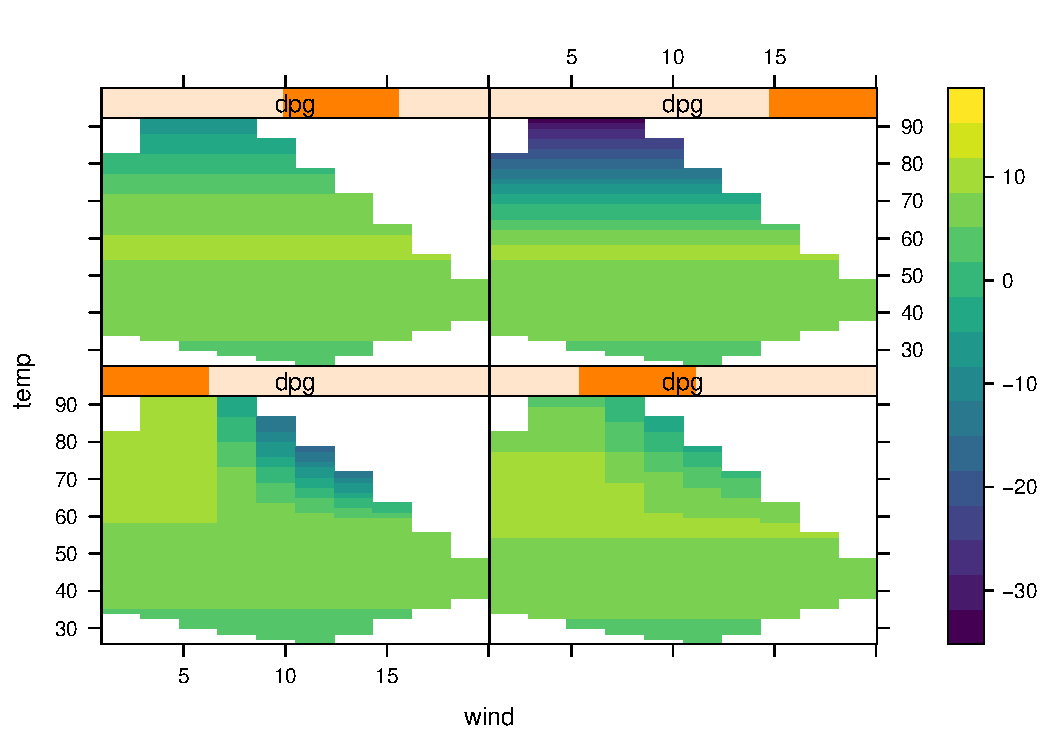
\includegraphics[width=0.8\linewidth]{partial_par}
  \caption{Partial dependence of \code{cmedv} on \code{lstat}, \code{rm}, and \code{ptratio}. Since \code{ptratio} is contiuous, it is first converted to a shingle; in this case, four groups with with 10\% overlap.}
  \label{fig:partial_par}
\end{figure}

\subsection{Classification problems}

For classification problems, partial dependence functions are on a scale similar to the logit; see, for example, \citet[pp. 369--370]{hastie-elements-2009}. Suppose the response is categorical with $K$ levels, then for each class we compute
\begin{equation}
\label{eqn:avg-logit}
f_k(x) = \log\left[p_k(x)\right] - \frac{1}{K}\sum_{i = 1}^K\log\left[p_k(x)\right], \quad k = 1, 2, \dots, K,
\end{equation}
where $p_k(x)$ is the predicted probability for the $k$-th class. Plotting $f_k(x)$ helps us understand how the log-odds for the $k$-th class depends on different subsets of the predictor variables.

To illustrate, consider Edgar Anderson's iris data from the \pkg{datasets} package. The \code{iris} data frame contains the sepal length, sepal width, petal length, and petal width (in centimeters) for 50 flowers from each of three species of iris:  setosa, versicolor, and virginica. We fit a support vector machine with a radial basis function kernel to the data usinv the \code{svm} function in the \pkg{e1071} (the model parameters were determined using 5-fold cross-validation).
\begin{example}
library(e1071)
iris.svm <- svm(Species ~ ., data = iris, kernel = "radial", gamma = 0.75,
                cost = 0.25, probability = TRUE)
\end{example}
The \code{partial} function has to be able to extract the predicted probabilities for each class, so it is necessary to invoke the \code{prob.model = TRUE} option in the call to \code{svm}.

Next, we plot the partial dependence of \code{Species} on both \code{Petal.Width} and \code{Petal.Length} for each of the three classes. The result is displayed in Figure~\ref{fig:partial_iris}.
\begin{example}
pd <- NULL
for (i in 1:3) {
  tmp <- partial(iris.svm, pred.var = c("Petal.Width", "Petal.Length"),
                 which.class = i, train = iris)
  pd <- rbind(pd, cbind(tmp, Species = levels(iris$Species)[i]))
}
lattice::levelplot(y ~ Petal.Width * Petal.Length | Species, data = pd)
\end{example}

\begin{figure}[htbp]
  \centering
  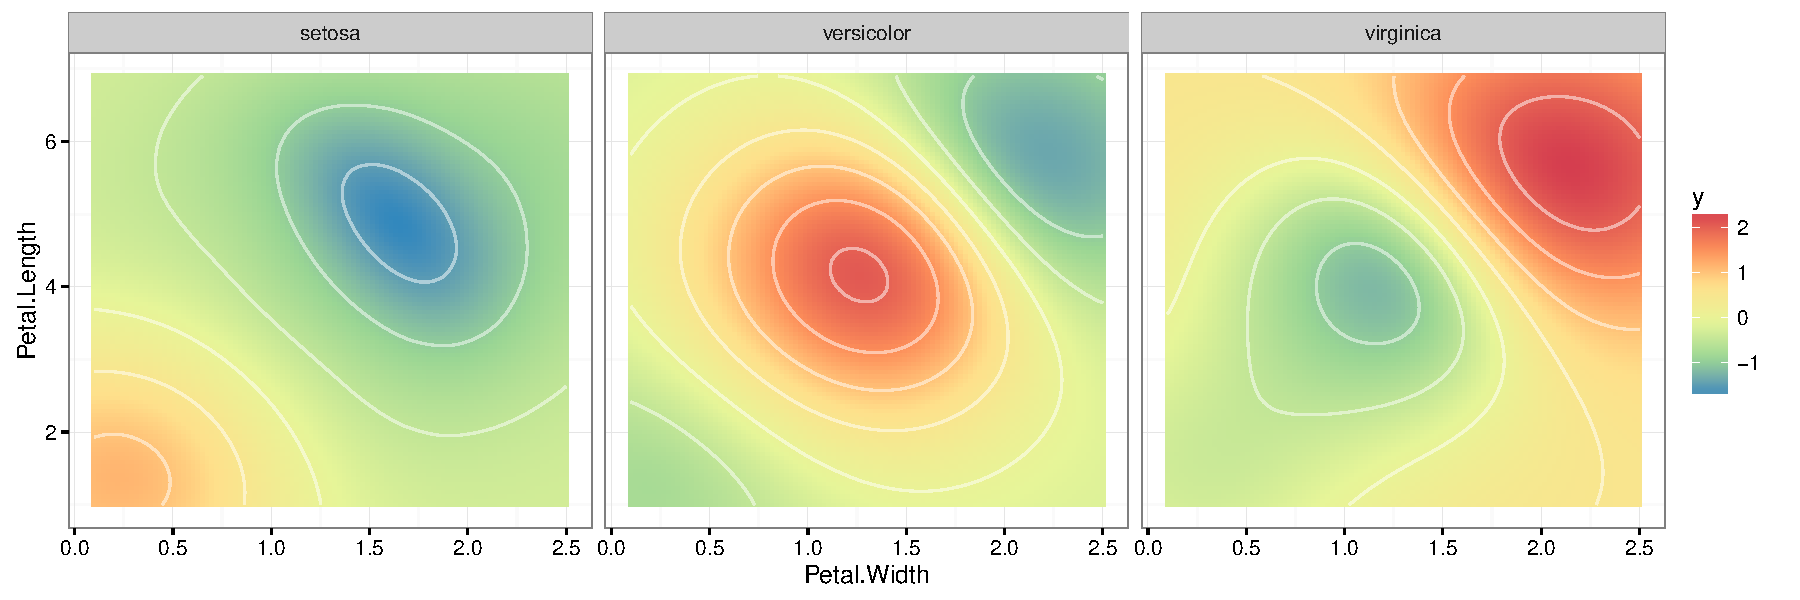
\includegraphics[width=1.0\linewidth]{partial_iris_svm}
  \caption{Partial dependence of species on petal width and petal length for the iris data.}
  \label{fig:partial_iris}
\end{figure}


%%%%%%%%%%%%%%%%%%%%%%%%%%%%%%%%%%%%%%%%%%%%%%%%%%%%%%%%%%%%%%%%%%%%%%%%%%%%%%%%
% Summary
%%%%%%%%%%%%%%%%%%%%%%%%%%%%%%%%%%%%%%%%%%%%%%%%%%%%%%%%%%%%%%%%%%%%%%%%%%%%%%%%
\section{Summary}

In this paper, we showed how to construct PDPs for various types of black box models in R using the \pkg{partial} package. We discussed similar approaches in other packages. Ways to avoid extrpolation and high excecution times were demonstrated via examples. There is a bright future for \pkg{partial} in terms of growth. For example, we would like to include the ability to construct PDPs for various types of survival models (e.g. conditional random forests with censored response).


%%%%%%%%%%%%%%%%%%%%%%%%%%%%%%%%%%%%%%%%%%%%%%%%%%%%%%%%%%%%%%%%%%%%%%%%%%%%%%%%
% Summary
%%%%%%%%%%%%%%%%%%%%%%%%%%%%%%%%%%%%%%%%%%%%%%%%%%%%%%%%%%%%%%%%%%%%%%%%%%%%%%%%
\section{Acknowledgments}

TBD.

%%%%%%%%%%%%%%%%%%%%%%%%%%%%%%%%%%%%%%%%%%%%%%%%%%%%%%%%%%%%%%%%%%%%%%%%%%%%%%%%
% Back matter
%%%%%%%%%%%%%%%%%%%%%%%%%%%%%%%%%%%%%%%%%%%%%%%%%%%%%%%%%%%%%%%%%%%%%%%%%%%%%%%%

\bibliography{greenwell}

\address{Brandon M. Greenwell\\
  Infoscitex Corporation\\
  4027 Colonel Glenn Highway\\
  Suite 210\\
  Dayton, OH 45431-1672\\
  United States of America\\}
\email{bgreenwell@infoscitex.com}
